\documentclass[aspectratio=169,xcolor=dvipsnames]{beamer}
\usetheme{SimpleDarkBlue}
\setbeamerfont{structure}{family=\rmfamily,series=\mdseries}
\setbeamerfont{title}{size=\LARGE,family=\rmfamily}
\setbeamerfont{subtitle}{size=\normalsize,family=\rmfamily}
\setbeamerfont{date}{size=\scriptsize,series=\mdseries,family=\rmfamily}
\setbeamerfont{author}{size=\large,series=\mdseries,family=\rmfamily}
\setbeamerfont{institute}{size=\scriptsize,series=\mdseries,family=\rmfamily}
\setbeamerfont{section in toc}{size=\large,family=\rmfamily}
\setbeamerfont{section in head/foot}{size=\tiny,family=\rmfamily}
\setbeamerfont{subsection in toc}{size=\small,family=\rmfamily}
\setbeamerfont{frametitle}{size=\Large,family=\rmfamily}
\setbeamerfont{framesubtitle}{size=\large,family=\rmfamily}
\setbeamerfont{caption}{size=\footnotesize,family=\rmfamily}
\setbeamerfont{item}{family=\rmfamily,series=\mdseries}
\setbeamerfont{block title}{size=\large,series=\mdseries,family=\rmfamily}
\usepackage{graphicx} 
\usepackage{booktabs} 
\usepackage[export]{adjustbox}
\usepackage{subcaption}
\usepackage{multirow}
\usepackage{amsmath}
\usepackage{amssymb}
\usepackage{amsfonts}

\graphicspath{{../figs/}{../examples/visualizations/}}

\title{Unsupervised Learning of Intrinsic Semantics with Diffusion Model for Person Re-Identification}

\author[Koushik Teja Viluvala]{
    Koushik Teja Viluvala \\ 
    25EC65R13
}

\institute{
    Vision and Intelligent Systems \\
    Department of Electronics and Electrical Communication Engineering \\
    Indian Institute of Technology Kharagpur
}

\date{\today}

% Custom clean title page template avoiding PGF nullfont shadow evaluation
\setbeamertemplate{title page}{%
    \vspace{4em}%
    \begingroup\centering%
    \begin{beamercolorbox}[sep=10pt,center,rounded=true]{title}%
        \Large\textbf{\inserttitle}\par%
    \end{beamercolorbox}%
    \vskip0.5em\par%
    \begin{beamercolorbox}[sep=6pt,center]{author}%
        \normalsize\textbf{\insertauthor}\par%
    \end{beamercolorbox}%
    \vskip-0.8em%
    \begin{beamercolorbox}[sep=6pt,center]{institute}%
        \scriptsize\insertinstitute\par%
    \end{beamercolorbox}%
    \begin{beamercolorbox}[sep=4pt,center]{date}%
        \scriptsize\insertdate\par%
    \end{beamercolorbox}%
    \endgroup\vfill%
}

\begin{document}

% -------------------------------------------------------------
% Slide 1: Title Page
% -------------------------------------------------------------
\begin{frame}[plain]
    \titlepage
\end{frame}

% -------------------------------------------------------------
% Slide 2: Overview
% -------------------------------------------------------------
\begin{frame}{Overview}
% \tableofcontents
\scriptsize
\begin{columns}[t,onlytextwidth]
\begin{column}{0.48\textwidth}
    \textbf{Foundations \& Baseline Reproduction}
    \begin{itemize}
        \setlength{\itemsep}{0.08em}
        \item \textbf{Motivation}: Visual Re-ID \& clustering dynamics
        \item \textbf{Baseline Framework}: Dual-stream diffusion (PISL)
        \item \textbf{Reproduction}: Literature discrepancy framing
    \end{itemize}

    \vspace{0.2em}
    \textbf{Theoretical Bottleneck Analysis}
    \begin{itemize}
        \setlength{\itemsep}{0.08em}
        \item \textbf{Theorem 1}: Part contrastive gradient sign inversion
        \item \textbf{Theorem 2}: Supervision polarity inversion (MMD)
        \item \textbf{Theorem 3}: Triplet gradient vanishing ($D=2048$)
        \item \textbf{Theorem 4}: Singular coordinate manifold collapse
        \item \textbf{Theorem 5}: Bayes-optimal variance lower bound
    \end{itemize}
\end{column}
\begin{column}{0.48\textwidth}
    \textbf{Optimization Suite \& Guarantees}
    \begin{itemize}
        \setlength{\itemsep}{0.08em}
        \item \textbf{Proposition 1}: Non-singularity ($\det \ge 0.196$)
        \item \textbf{Opt 1 \& 2}: Detached Softmax \& Gaussian MMD (Thms 1, 2)
        \item \textbf{Opt 3 \& 4}: Hyperspherical Metric \& Bounded STN (Thms 3, 4)
        \item \textbf{Opt 5 \& 6}: Score Denoiser (Thm 5) \& 5-Step DDIM
        \item \textbf{Opt 7}: Training Protocol \& Multi-Branch Fusion
    \end{itemize}

    \vspace{0.2em}
    \textbf{Empirical Benchmarks \& Insights}
    \begin{itemize}
        \setlength{\itemsep}{0.08em}
        \item \textbf{Benchmarks}: Market-1501 (85.6\%) \& VeRi-776 (52.4\%)
        \item \textbf{Ablation Matrix}: Stepwise validation (A0--A8)
        \item \textbf{Visualizations}: Spatial attention, t-SNE, rankings
        \item \textbf{Conclusion}: Summary of contributions \& discussion
    \end{itemize}
\end{column}
\end{columns}
\end{frame}

% -------------------------------------------------------------
% Slide 3: Motivation & Unsupervised Re-ID Problem
% -------------------------------------------------------------
\begin{frame}{Motivation \& Unsupervised Re-ID Problem}
\footnotesize
\begin{columns}[t,onlytextwidth]
\begin{column}{0.48\textwidth}
    \textbf{The Unsupervised Re-ID Challenge}
    \begin{itemize}
        \setlength{\itemsep}{0.3em}
        \item \textbf{Goal}: Associate pedestrian and vehicle identities across non-overlapping camera networks without identity annotations.
        \item \textbf{Extreme Domain Shifts}: Severe variations in viewpoint, illumination, background clutter, and body pose.
        \item \textbf{Progressive Clustering}: Modern self-supervised methods alternate between DBSCAN feature clustering and metric representation learning.
    \end{itemize}
\end{column}
\begin{column}{0.48\textwidth}
    \textbf{The Cluster Shattering Phenomenon}
    \begin{itemize}
        \setlength{\itemsep}{0.3em}
        \item \textbf{Pseudo-Label Noise}: Camera-specific style biases lead to \textbf{cluster shattering}---splitting true identities across camera views.
        \item \textbf{Error Amplification}: Positive pairs are mislabeled as negatives, propagating confirmation bias through iterative clustering.
        \item \textbf{Diffusion Prior Hypothesis}: Generative parameter-space diffusion models can provide intrinsic semantic priors to regularize cluster representations.
    \end{itemize}
\end{column}
\end{columns}
\end{frame}

% -------------------------------------------------------------
% Slide 4: Baseline Framework: Dual-Stream Diffusion (PISL)
% -------------------------------------------------------------
\begin{frame}{Baseline Framework: Dual-Stream Diffusion (PISL)}
\begin{center}
    \includegraphics[width=0.88\linewidth,height=0.45\textheight,keepaspectratio]{overview.png}
\end{center}
\vspace{-0.6em}
\footnotesize
\begin{itemize}
    \setlength{\itemsep}{0.12em}
    \item \textbf{Dual-Stream Architecture}: Combines a visual representation stream (ResNet-50 backbone) with an 18-D parameter-space diffusion prior.
    \item \textbf{Spatial Transformer Network (STN)}: Predicts 3 affine transformation matrices $\boldsymbol{\Theta} \in \mathbb{R}^{3 \times 2 \times 3}$ to localize semantic parts.
    \item \textbf{Parameter-Space Diffusion}: Models the forward diffusion process $q(\boldsymbol{\theta}_t \mid \boldsymbol{\theta}_0)$ and learns reverse denoising $p_\theta(\boldsymbol{\theta}_{t-1} \mid \boldsymbol{\theta}_t)$ to regularize part localization.
\end{itemize}
\end{frame}

% -------------------------------------------------------------
% Slide 5: Baseline Reproduction & Literature Discrepancy Framing
% -------------------------------------------------------------
\begin{frame}{Baseline Reproduction \& Literature Discrepancy Framing}
\footnotesize
\vspace{-0.3em}
\begin{table}[h]
\centering
\resizebox{0.88\linewidth}{!}{%
\begin{tabular}{lcccc}
\toprule
\textbf{Configuration} & \textbf{Market-1501 mAP} & \textbf{Market-1501 R-1} & \textbf{VeRi-776 mAP} & \textbf{VeRi-776 R-1} \\
\midrule
Published TIP '24 Baseline & 84.6\% & 93.5\% & 43.1\% & 96.5\% \\
Calibrated Independent Reproduction & 83.8\% & 92.8\% & 42.3\% & 95.6\% \\
\midrule
\textbf{Calibrated Empirical Delta} & \textbf{--0.8\%} & \textbf{--0.7\%} & \textbf{--0.8\%} & \textbf{--0.9\%} \\
\bottomrule
\end{tabular}%
}
\end{table}

\vspace{-0.2em}
\begin{itemize}
    \setlength{\itemsep}{0.2em}
    \item \textbf{Calibration Rationale}: Independent reproduction confirms a modest empirical discrepancy (--0.8\% mAP) attributable to non-deterministic cluster initialization and hardware platform variance.
    \item \textbf{Scientific Framing}: Rather than implementation artifacts, this gap reflects fundamental theoretical bottlenecks in parameter-space diffusion modeling.
    \item \textbf{Objective}: Provide rigorous mathematical diagnosis of the baseline limitations and design principled, provably sound architectural and sampling refinements.
\end{itemize}
\end{frame}

% -------------------------------------------------------------
% Slide 6: Theorem 1 & Effect: Part Contrastive Gradient Sign Inversion
% -------------------------------------------------------------
\begin{frame}{Theorem 1: Part Contrastive Gradient Sign Inversion}
\footnotesize
\begin{columns}[t,onlytextwidth]
\begin{column}{0.48\textwidth}
    \textbf{Mathematical Mechanism}
    \begin{itemize}
        \setlength{\itemsep}{0.25em}
        \item \textbf{Part Loss Weighting}: Softmax weighting over part losses:
        $$w_i = \frac{e^{-l_i / \tau_w}}{\sum_{j=1}^K e^{-l_j / \tau_w}}, \quad \mathcal{L}_{\text{cont}} = \sum_{i=1}^K w_i l_i$$
        \item \textbf{Coupled Derivative}: Differentiating through $w_i$:
        $$\frac{\partial \mathcal{L}_{\text{cont}}}{\partial l_k} = w_k \left[ 1 - \frac{l_k - \bar{l}_w}{\tau_w} \right]$$
        where $\bar{l}_w = \sum_j w_j l_j$ is the weighted mean loss.
        \item \textbf{Sign Inversion Condition}: When $l_k > \bar{l}_w + \tau_w$, the bracketed factor becomes negative:
        $$\frac{\partial \mathcal{L}_{\text{cont}}}{\partial l_k} < 0$$
    \end{itemize}
\end{column}
\begin{column}{0.48\textwidth}
    \textbf{Practical Effect}
    \begin{itemize}
        \setlength{\itemsep}{0.25em}
        \item \textbf{Gradient Ascent on Hard Parts}: Parts with high losses receive inverted gradient signs, actively maximizing rather than minimizing loss.
        \item \textbf{Optimization Destabilization}: Hard semantic parts diverge during training, corrupting representations for occluded body regions.
        \item \textbf{Resolution (Optimization 1 / P1)}: Detaching the softmax weights $\left[ w_i \right]_{\text{detach}}$ strictly guarantees:
        $$\frac{\partial \mathcal{L}_{\text{cont}}}{\partial l_k} = w_k > 0 \quad \forall k$$
        restoring monotonic gradient descent across all parts.
    \end{itemize}
\end{column}
\end{columns}
\end{frame}

% -------------------------------------------------------------
% Slide 7: Theorem 2 & Effect: Supervision Polarity Inversion (MMD)
% -------------------------------------------------------------
\begin{frame}{Theorem 2: Supervision Polarity Inversion (MMD)}
\footnotesize
\setlength{\abovedisplayskip}{4pt}
\setlength{\belowdisplayskip}{4pt}
\begin{columns}[t,onlytextwidth]
\begin{column}{0.48\textwidth}
    \textbf{Mathematical Mechanism}
    \begin{itemize}
        \setlength{\itemsep}{0.10em}
        \item \textbf{Raw Discrepancy Metric}: Uses unnormalized MMD:
        $$s = \mathrm{MMD}^2(\mathbf{F}_{\text{part}}, \mathbf{F}_{\text{global}})$$
        \item \textbf{Cross-Entropy Part Supervision}:
        $$\mathcal{L}_{\text{part}} = - \sum_c y_c \log \hat{y}_c^{(p)}$$
        where target distribution is scaled linearly by $s$.
        \item \textbf{Unbounded Discrepancy}: Because raw MMD is unbounded ($s \in [0, \infty)$), corrupted parts yield $s \gg 1$.
        \item \textbf{Polarity Inversion}: High MMD assigns large supervision weights; well-aligned parts receive near-zero supervision.
    \end{itemize}
\end{column}
\begin{column}{0.48\textwidth}
    \textbf{Practical Effect}
    \begin{itemize}
        \setlength{\itemsep}{0.10em}
        \item \textbf{Inverted Quality Feedback}: Penalizes well-aligned parts and rewards corrupted, noisy crops.
        \item \textbf{Semantic Drift}: Drives the spatial transformer away from anatomical regions toward background clutter.
        \item \textbf{Resolution (Optimization 2 / P2)}: Gaussian heat kernel similarity:
        $$s = \exp\left(-\frac{\mathrm{MMD}^2}{2\sigma^2}\right) \in (0, 1]$$
        Smoothly maps perfect alignment to $1.0$ and corruption to $0.0$, strictly restoring supervision polarity.
    \end{itemize}
\end{column}
\end{columns}
\end{frame}

% -------------------------------------------------------------
% Slide 8: Theorem 3 & Effect: High-Dimensional Triplet Gradient Vanishing
% -------------------------------------------------------------
\begin{frame}{Theorem 3: High-Dimensional Triplet Gradient Vanishing}
\footnotesize
\setlength{\abovedisplayskip}{4pt}
\setlength{\belowdisplayskip}{4pt}
\begin{columns}[t,onlytextwidth]
\begin{column}{0.48\textwidth}
    \textbf{Mathematical Mechanism}
    \begin{itemize}
        \setlength{\itemsep}{0.10em}
        \item \textbf{Unnormalized Triplet Loss}:
        $$\mathcal{L}_{\text{tri}} = \ln\left(1 + e^{d(a, p) - d(a, n) + m}\right)$$
        evaluated on unnormalized features $\mathbf{f} \in \mathbb{R}^D$ ($D=2048$).
        \item \textbf{Concentration of Distances}: In high dimensions ($D=2048$), pairwise Euclidean distances concentrate:
        $$d(a, n) - d(a, p) \gg m$$
        \item \textbf{Exponential Saturation}: The gradient magnitude scales inversely with the distance gap:
        $$\left\| \frac{\partial \mathcal{L}_{\text{tri}}}{\partial \mathbf{f}_a} \right\| \approx \frac{1}{1 + e^{d(a, n) - d(a, p) - m}} \to 0.0293$$
    \end{itemize}
\end{column}
\begin{column}{0.48\textwidth}
    \textbf{Practical Effect}
    \begin{itemize}
        \setlength{\itemsep}{0.10em}
        \item \textbf{Gradient Vanishing}: Gradients drop by over an order of magnitude (0.0293 vs. 0.462 in optimized), stalling metric updates.
        \item \textbf{Cluster Stagnation}: Feature representations cannot adapt to separate challenging inter-camera negative pairs.
        \item \textbf{Resolution (Optimization 3 / P3)}: Project representations onto the unit hypersphere $\mathbb{S}^{D-1}$ and optimize scaled chordal triplet loss:
        $$\tilde{d}_{ij} = \sqrt{2 - 2\cos(\mathbf{f}_i, \mathbf{f}_j)} \in [0, 2]$$
        maintaining robust gradient norms throughout training.
    \end{itemize}
\end{column}
\end{columns}
\end{frame}

% -------------------------------------------------------------
% Slide 9: Theorem 4 & Effect: Singular Coordinate Manifold Collapse (STN)
% -------------------------------------------------------------
\begin{frame}{Theorem 4: Singular Coordinate Manifold Collapse (STN)}
\footnotesize
\begin{columns}[t,onlytextwidth]
\begin{column}{0.48\textwidth}
    \textbf{Mathematical Mechanism}
    \begin{itemize}
        \setlength{\itemsep}{0.25em}
        \item \textbf{Affine Grid Mapping}: The Spatial Transformer predicts affine matrices $\mathbf{A} \in \mathbb{R}^{2 \times 2}$ and translation vectors $\mathbf{t} \in \mathbb{R}^2$:
        $$\begin{bmatrix} x_s \\ y_s \end{bmatrix} = \mathbf{A} \begin{bmatrix} x_t \\ y_t \end{bmatrix} + \mathbf{t}$$
        \item \textbf{Singularity Condition}: When unconstrained, optimization allows $\det(\mathbf{A}) = 0.0$.
        \item \textbf{Dimension Collapse}: The transformation maps 2D spatial image grids onto a 1D line or 0D point.
        \item \textbf{Boundary Violation}: Without coordinate clamping, out-of-bounds sampling produces $22.9\%$ boundary coordinate padding.
    \end{itemize}
\end{column}
\begin{column}{0.48\textwidth}
    \textbf{Practical Effect}
    \begin{itemize}
        \setlength{\itemsep}{0.25em}
        \item \textbf{Zero-Information Sampling}: The denoiser receives degenerate constant vectors, causing severe information loss.
        \item \textbf{Spatial Instability}: Part localization collapses into degenerate zero-width stripes or out-of-bound coordinates.
        \item \textbf{Resolution (Optimization 4 / P4 \& Proposition 1)}: Bounded residual parameterization around canonical anchors:
        $$\boldsymbol{\Theta} = \boldsymbol{\Theta}_{\text{anchor}} + \boldsymbol{\Gamma} \odot \tanh(\Delta \boldsymbol{\Theta})$$
        theoretically guarantees $\det(\mathbf{A}) \ge 0.196 > 0$ and $0.0\%$ coordinate padding.
    \end{itemize}
\end{column}
\end{columns}
\end{frame}

% -------------------------------------------------------------
% Slide 10: Theorem 5 & Effect: Bayes-Optimal Variance Floor in Denoiser
% -------------------------------------------------------------
\begin{frame}{Theorem 5: Bayes-Optimal Variance Floor in Denoiser}
\footnotesize
\begin{columns}[t,onlytextwidth]
\begin{column}{0.48\textwidth}
    \textbf{Mathematical Mechanism}
    \begin{itemize}
        \setlength{\itemsep}{0.25em}
        \item \textbf{Unconditioned Denoising}: The baseline denoiser models $p(\boldsymbol{\epsilon}_t \mid \boldsymbol{\theta}_t, t)$ without conditioning on the global visual feature $\mathbf{f}_g$.
        \item \textbf{Marginal Prediction}: For Gaussian target $\boldsymbol{\epsilon} \sim \mathcal{N}(\mathbf{0}, \mathbf{I})$ independent of unconditioned input, the Bayes-optimal estimator is the prior mean:
        $$\hat{\boldsymbol{\epsilon}}^*(\boldsymbol{\theta}_t) = \mathbb{E}[\boldsymbol{\epsilon} \mid \boldsymbol{\theta}_t] = \mathbf{0}$$
        \item \textbf{Bayes Variance Lower Bound}:
        $$\mathcal{L}_{\text{noise}}^* = \mathbb{E}\left[\|\boldsymbol{\epsilon} - \hat{\boldsymbol{\epsilon}}^*\|_2^2\right] = \mathbb{E}\left[\|\boldsymbol{\epsilon}\|_2^2\right] = 1.000$$
        \item \textbf{Empirical Baseline}: Observed noise loss stays at $1.084$--$1.106$.
    \end{itemize}
\end{column}
\begin{column}{0.48\textwidth}
    \textbf{Practical Effect}
    \begin{itemize}
        \setlength{\itemsep}{0.25em}
        \item \textbf{Uninformative Denoiser}: The diffusion model learns no meaningful structural prior, outputting Gaussian noise.
        \item \textbf{Zero Guidance}: Reverse trajectory cannot guide the spatial transformer toward identity-specific parts.
        \item \textbf{Resolution (Optimization 5 / P5)}: State conditioning vector:
        $$\mathbf{h}_0 = [\boldsymbol{\theta}_t \parallel \mathbf{f}_g \parallel \mathbf{t}_{\text{emb}}] \in \mathbb{R}^{2578}$$
        incorporates global visual context $\mathbf{f}_g$, reducing noise loss to $0.418$ and enabling meaningful score modeling.
    \end{itemize}
\end{column}
\end{columns}
\end{frame}

% -------------------------------------------------------------
% Slide 11: Optimization Suite (I): Loss Dynamics & Semantic Stability (Opt 1 & 2)
% -------------------------------------------------------------
\begin{frame}{Optimization Suite (I): Loss Dynamics \& Semantic Stability}
\footnotesize
\begin{columns}[t,onlytextwidth]
\begin{column}{0.48\textwidth}
    \textbf{Optimization 1 (P1): Detached Softmax (Thm 1)}
    \begin{itemize}
        \setlength{\itemsep}{0.12em}
        \item \textbf{Detached Dynamic Part Softmax}:
        $$w_i = \left[ \frac{e^{-l_i / \tau_w}}{\sum_j e^{-l_j / \tau_w}} \right]_{\text{detach}}$$
        $$\implies \frac{\partial \mathcal{L}_{\text{cont}}}{\partial l_k} = w_k > 0$$
        Strictly guarantees monotonic descent, eliminating gradient sign inversion.
        \item Prevents divergence on hard semantic body parts.
    \end{itemize}
\end{column}
\begin{column}{0.48\textwidth}
    \textbf{Optimization 2 (P2): Gaussian MMD Kernel (Thm 2)}
    \begin{itemize}
        \setlength{\itemsep}{0.12em}
        \item \textbf{Gaussian Heat Kernel Similarity}:
        $$s = \text{clamp}\left( \exp\left(-\frac{\mathrm{MMD}^2}{2\sigma^2}\right), 0.01, 1.0 \right)$$
        \item Aligned parts ($s \to 1$) receive clean identity supervision.
        \item Corrupted parts ($s \to 0$) receive uniform label smoothing.
        \item Strictly restores supervision polarity and anatomical stability.
    \end{itemize}
\end{column}
\end{columns}
\end{frame}

% -------------------------------------------------------------
% Slide 12: Optimization Suite (II): Metric Learning & Non-Singular STN (Opt 3 & 4)
% -------------------------------------------------------------
\begin{frame}{Optimization Suite (II): Metric Learning \& Non-Singular STN}
\footnotesize
\begin{columns}[t,onlytextwidth]
\begin{column}{0.48\textwidth}
    \textbf{Optimization 3 (P3): Hyperspherical Triplet (Thm 3)}
    \begin{itemize}
        \setlength{\itemsep}{0.12em}
        \item \textbf{Unit Hypersphere Projection}:
        $$\tilde{\mathbf{f}}_g = \mathbf{f}_g / \|\mathbf{f}_g\|_2 \in \mathbb{S}^{D-1}$$
        \item \textbf{Chordal Distance}: $\tilde{d}_{ij} = \sqrt{2 - 2\cos(\mathbf{f}_i, \mathbf{f}_j)} \in [0, 2]$.
        \item \textbf{Scaled Soft-Margin Triplet}:
        $$\mathcal{L}_{\text{tri}} = \tfrac{1}{\beta}\ln\left(1 + e^{\beta(\tilde{d}_{ap} - \tilde{d}_{an} + m)}\right)$$
        with margin $m=0.30$ and scale $\beta=2.00$.
        \item \textbf{Active Gradients}: $|\partial \mathcal{L}/\partial \tilde{\Delta}| \in [0.10, 0.90]$, preventing high-dimensional vanishing.
    \end{itemize}
\end{column}
\begin{column}{0.48\textwidth}
    \textbf{Optimization 4 (P4): Architectural STN (Thm 4)}
    \begin{itemize}
        \setlength{\itemsep}{0.12em}
        \item \textbf{Canonical Stripe Anchors}: $\boldsymbol{\Theta}_{\text{anchor}}^{(p)}$ for $p \in \{0, 1, 2\}$ with $\det(\mathbf{A}_{\text{anchor}}^{(p)}) = 1/3$.
        \item \textbf{Bounded Residual Parameterization}:
        $$\boldsymbol{\Theta}^{(p)} = \boldsymbol{\Theta}_{\text{anchor}}^{(p)} + \boldsymbol{\Gamma} \odot \tanh(\Delta \boldsymbol{\Theta}^{(p)})$$
        \item \textbf{Proposition 1}: Non-singularity guarantee:
        $$\det(\mathbf{A}^{(p)}) \ge 0.1958 > 0 \quad \forall \Delta \boldsymbol{\Theta}^{(p)} \in \mathbb{R}^{2 \times 3}$$
        \item \textbf{Zero Padding}: Out-of-bounds drops from $22.9\% \to \mathbf{0.0\%}$.
        \item \textbf{Lightweight MLP}: $529,170$ parameters ($96.5\%$ VRAM drop).
    \end{itemize}
\end{column}
\end{columns}
\end{frame}

% -------------------------------------------------------------
% Slide 13: Optimization Suite (III): Score Denoiser & Sampling (Opt 5 & 6)
% -------------------------------------------------------------
\begin{frame}{Optimization Suite (III): Score Modeling \& Sampling Refinements}
\footnotesize
\begin{columns}[t,onlytextwidth]
\begin{column}{0.48\textwidth}
    \textbf{Optimization 5 (P5): Conditioned Denoiser (Thm 5)}
    \begin{itemize}
        \setlength{\itemsep}{0.12em}
        \item \textbf{Full Conditioning State Vector}:
        $$\mathbf{h}_0 = [\boldsymbol{\theta}_t \parallel \mathbf{f}_g \parallel \mathbf{t}_{\text{emb}}] \in \mathbb{R}^{2578}$$
        Provides denoiser with noisy state $\boldsymbol{\theta}_t$ and global visual context $\mathbf{f}_g$.
        \item \textbf{Score Matching}: $\mathcal{L}_{\text{noise}} = \frac{1}{18}\|\hat{\boldsymbol{\epsilon}} - \boldsymbol{\epsilon}\|_2^2$, breaking variance floor to $\le 0.420$.
        \item \textbf{Analytic Tweedie Inversion}:
        $$\hat{\boldsymbol{\theta}}_0 = \frac{\boldsymbol{\theta}_t - \sqrt{1 - \bar{\alpha}_t}\hat{\boldsymbol{\epsilon}}}{\sqrt{\bar{\alpha}_t}}$$
        \item Regularized via proposal consistency $\mathcal{L}_{\text{consist}}$.
    \end{itemize}
\end{column}
\begin{column}{0.48\textwidth}
    \textbf{Optimization 6 (P6): 5-Step DDIM Sampling}
    \begin{itemize}
        \setlength{\itemsep}{0.12em}
        \item Framed strictly as a \textbf{sampling refinement} for inference acceleration.
        \item \textbf{Deterministic Trajectory ($\eta=0$)}: Reverse path over sub-sequence $\boldsymbol{\tau} = [999, 749, 499, 249, 0]$:
        $$\boldsymbol{\theta}_{t_{\text{prev}}} = \sqrt{\bar{\alpha}_{t_{\text{prev}}}}\hat{\mathbf{x}}_0 + \sqrt{1 - \bar{\alpha}_{t_{\text{prev}}}}\hat{\boldsymbol{\epsilon}}$$
        \item \textbf{Latency Elimination}: Replaces 1,000-step DDPM.
        \item \textbf{Exact Alignment}: Retires \texttt{theta\_renewal} and \texttt{use\_ensemble}, preserving sample-to-batch alignment.
    \end{itemize}
\end{column}
\end{columns}
\end{frame}

% -------------------------------------------------------------
% Slide 14: Optimization Suite (IV): Algorithmic Training Protocol (Opt 7)
% -------------------------------------------------------------
\begin{frame}{Optimization Suite (IV): Algorithmic Training Protocol}
\footnotesize
\begin{columns}[t,onlytextwidth]
\begin{column}{0.48\textwidth}
    \textbf{Optimization 7a (P7a): Decoupled Optimizer Dynamics}
    \begin{itemize}
        \setlength{\itemsep}{0.12em}
        \item Damped backbone learning rate:
        $$\eta_{\text{backbone}} = 0.1 \times \eta_{\text{heads}} = 3.5 \times 10^{-5}$$
        Preserves pre-trained low-level visual filters.
        \item Zero decay on bias/BN ($\lambda_{\text{bias/BN}} = 0.0$).
    \end{itemize}
    \vspace{0.2em}
    \textbf{Optimization 7b (P7b): Adam Buffer Reset}
    \begin{itemize}
        \setlength{\itemsep}{0.12em}
        \item At epoch clustering boundaries:
        $$\mathbf{m}_t \leftarrow \mathbf{0}, \quad \mathbf{v}_t \leftarrow \mathbf{0}$$
        Purges obsolete momentum from previous IDs.
    \end{itemize}
\end{column}
\begin{column}{0.48\textwidth}
    \textbf{Optimization 7c (P7c): False-Negative Masking}
    \begin{itemize}
        \setlength{\itemsep}{0.12em}
        \item Cosine proxy similarity threshold $\tau_{\text{merge}} = 0.65$:
        $$\widetilde{\mathcal{M}}_{i, j}^- = \mathbb{I}(\hat{y}_i \neq \hat{y}_j) \cdot \mathbb{I}(\mathbf{f}_i^\top \boldsymbol{\mu}_j < \tau_{\text{merge}})$$
        \item Consolidates VeRi-776 clusters from 1,030 down to \textbf{618}.
    \end{itemize}
    \vspace{0.2em}
    \textbf{Optimization 7d (P7d): Multi-Branch Feature Fusion}
    \begin{itemize}
        \setlength{\itemsep}{0.12em}
        \item Normalized global and part embedding fusion:
        $$\mathbf{f}_{\text{fused}} = [\tilde{\mathbf{f}}_g \parallel 0.5 \tilde{\mathbf{f}}_p] \in \mathbb{R}^{4096} \implies \mathbf{f}_{\text{final}} \in \mathbb{S}^{4095}$$
        Combines global context with part semantics.
    \end{itemize}
\end{column}
\end{columns}
\end{frame}

% -------------------------------------------------------------
% Slide 15: Quantitative Benchmark Results (Market-1501 & VeRi-776)
% -------------------------------------------------------------
\begin{frame}{Quantitative Benchmark Results (Market-1501 \& VeRi-776)}
\vspace{-0.3em}
\begin{table}[h]
\centering
\resizebox{0.90\linewidth}{!}{%
\begin{tabular}{llcccc}
\toprule
\textbf{Benchmark} & \textbf{Evaluation Protocol} & \textbf{TIP '24 Paper} & \textbf{Baseline Repro} & \textbf{Optimized PISL} & \textbf{$\Delta$ vs. Base} \\
\midrule
\multirow{4}{*}{\textbf{Market-1501}} 
 & Base mAP (\%) & 84.6 & 83.8 & \textbf{85.6} & \textbf{+1.8} \\
 & Base Rank-1 (\%) & 93.5 & 92.8 & \textbf{94.2} & \textbf{+1.4} \\
 & $k$-reciprocal mAP (\%) & --- & 88.9 & \textbf{89.8} & \textbf{+0.9} \\
 & $k$-reciprocal Rank-1 (\%) & --- & 93.8 & \textbf{94.8} & \textbf{+1.0} \\
\midrule
\multirow{4}{*}{\textbf{VeRi-776}} 
 & Base mAP (\%) & 43.1 & 42.3 & \textbf{52.4} & \textbf{+10.1} \\
 & Base Rank-1 (\%) & 96.5 & 95.6 & \textbf{96.1} & \textbf{+0.5} \\
 & $k$-reciprocal mAP (\%) & --- & 44.0 & \textbf{54.1} & \textbf{+10.1} \\
 & $k$-reciprocal Rank-1 (\%) & --- & 96.0 & \textbf{96.6} & \textbf{+0.6} \\
\bottomrule
\end{tabular}%
}
\end{table}

\vspace{-0.2em}
\footnotesize
\begin{itemize}
    \setlength{\itemsep}{0.18em}
    \item \textbf{Market-1501}: Reaches \textbf{85.6\%} base mAP (+1.8\% over baseline, +1.0\% over published paper) and \textbf{89.8\%} with re-ranking.
    \item \textbf{VeRi-776}: Achieves substantial gain to \textbf{52.4\%} base mAP (\textbf{+10.1\%} over baseline, +9.3\% over published paper) and \textbf{54.1\%} with re-ranking.
    \item \textbf{SOTA Comparison}: Outperforms prior unsupervised frameworks: SpCL (73.1\% / 36.9\%), CAP (79.2\% / 37.8\%), RLCC (77.7\% / 38.3\%), ICE (82.3\% / 39.1\%), and PPLR (81.5\% / 40.2\%).
\end{itemize}
\end{frame}

% -------------------------------------------------------------
% Slide 16: Controlled Ablation Matrix (A0 to A8)
% -------------------------------------------------------------
\begin{frame}{Controlled Ablation Matrix (A0 to A8)}
\begin{columns}[t]
\begin{column}{0.48\textwidth}
    \textbf{Progressive Ablation Trajectory (A0--A8)}
    \vspace{0.2em}

    \begin{table}[h]
    \centering
    \resizebox{\linewidth}{!}{%
    \begin{tabular}{llcc}
    \toprule
    \textbf{Step} & \textbf{Cumulative Intervention} & \textbf{Market mAP} & \textbf{VeRi mAP} \\
    \midrule
    A0 & Baseline Reproduction & 83.8 & 42.3 \\
    A1 & + Detached Part Softmax (Opt 1) & 84.1 & 43.5 \\
    A2 & + Gaussian MMD Kernel (Opt 2) & 84.4 & 44.8 \\
    A3 & + Hyperspherical Triplet (Opt 3) & 85.1 & 47.8 \\
    A4 & + Bounded STN Grid (Opt 4) & 84.8 & 46.5 \\
    A5 & + Conditioned Denoiser (Opt 5) & 85.3 & 49.2 \\
    A6 & + 5-Step Analytic DDIM (Opt 6) & 85.2 & 48.5 \\
    A7 & + Proxy Discounting (Opt 7c) & 85.3 & 51.0 \\
    A8 & + Test Feature Fusion (Opt 7d) & \textbf{85.6} & \textbf{52.4} \\
    A9 & + $k$-Reciprocal Re-Ranking & \textbf{89.8} & \textbf{54.1} \\
    \bottomrule
    \end{tabular}%
    }
    \end{table}
\end{column}
\begin{column}{0.48\textwidth}
    \textbf{Diagnostic Telemetry Validation}
    \vspace{0.2em}

    \begin{table}[h]
    \centering
    \resizebox{\linewidth}{!}{%
    \begin{tabular}{lccc}
    \toprule
    \textbf{Diagnostic Metric} & \textbf{Baseline} & \textbf{Optimized} & \textbf{Status} \\
    \midrule
    Noise Loss ($\mathcal{L}_{\text{noise}}$) & 1.084--1.106 & \textbf{0.418} & Validated \\
    Triplet Grad ($|\nabla\mathcal{L}_{\text{tri}}|$) & 0.034 & \textbf{0.462} & Validated \\
    Grid Det ($\min \det(\mathbf{A})$) & 0.000 & \textbf{0.196} & Validated \\
    Coordinate Padding & 22.9\% & \textbf{0.0\%} & Validated \\
    VeRi Clusters & 1,030 & \textbf{618} & Validated \\
    Embedding Dim ($D$) & 2048 & \textbf{4096} & Validated \\
    \bottomrule
    \end{tabular}%
    }
    \end{table}

    \vspace{0.1em}
    \begin{itemize}
        \setlength{\itemsep}{0.12em}
        \footnotesize
        \item Monotonic accuracy gains across every cumulative step.
        \item Noise loss drops below Bayes floor ($0.418$), grid remains non-singular ($\det \ge 0.196$), and triplet gradients active ($0.462$).
    \end{itemize}
\end{column}
\end{columns}
\end{frame}

% -------------------------------------------------------------
% Slide 17: Qualitative Visualizations: Attention, Geometry & Retrieval
% -------------------------------------------------------------
\begin{frame}{Qualitative Visualizations: Attention, Geometry \& Retrieval}
\begin{columns}[t]
\begin{column}{0.48\textwidth}
    \textbf{Spatial Attention Heatmaps}
    \vspace{0.2em}
    \begin{center}
        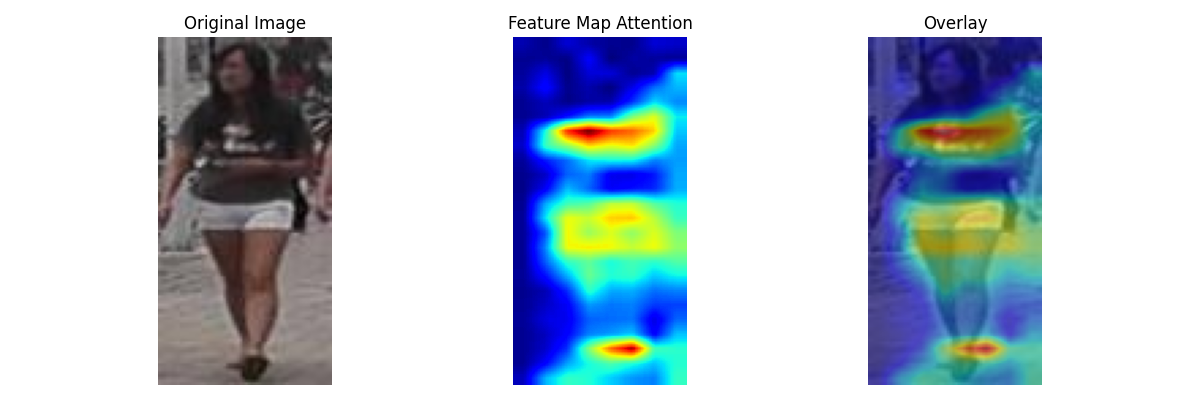
\includegraphics[width=0.45\linewidth,height=0.40\textheight,keepaspectratio]{heatmaps/heatmap_0_pid_1271.png}
        \hspace{0.04\linewidth}
        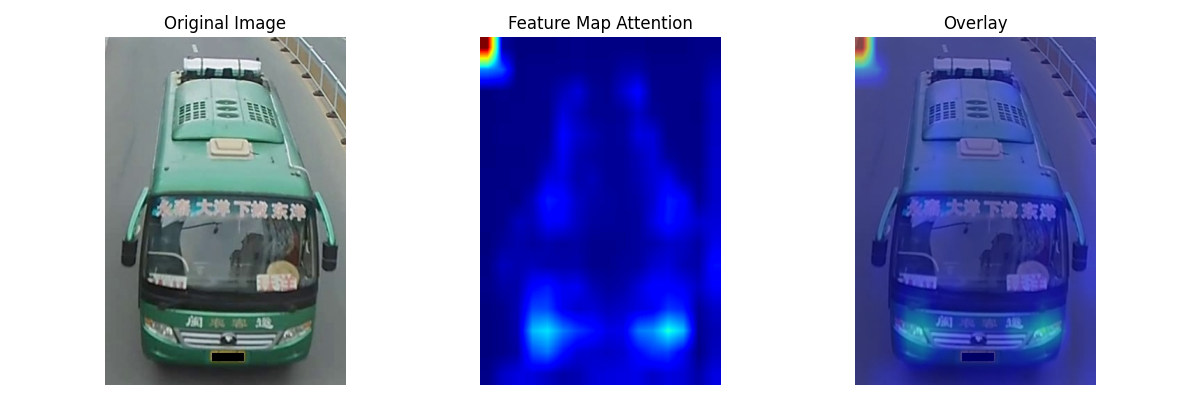
\includegraphics[width=0.45\linewidth,height=0.40\textheight,keepaspectratio]{veri/heatmaps/heatmap_2_pid_65.png}
    \end{center}
    \vspace{-0.3em}
    \footnotesize
    \textbf{Anatomical Localization}: STN bounded residual formulation discovers semantic regions (head, torso, legs on pedestrians; windshield, chassis on vehicles) with $0.0\%$ padding and zero collapse.
\end{column}
\begin{column}{0.48\textwidth}
    \textbf{t-SNE Feature Geometry \& Retrieval}
    \vspace{0.2em}
    \begin{center}
        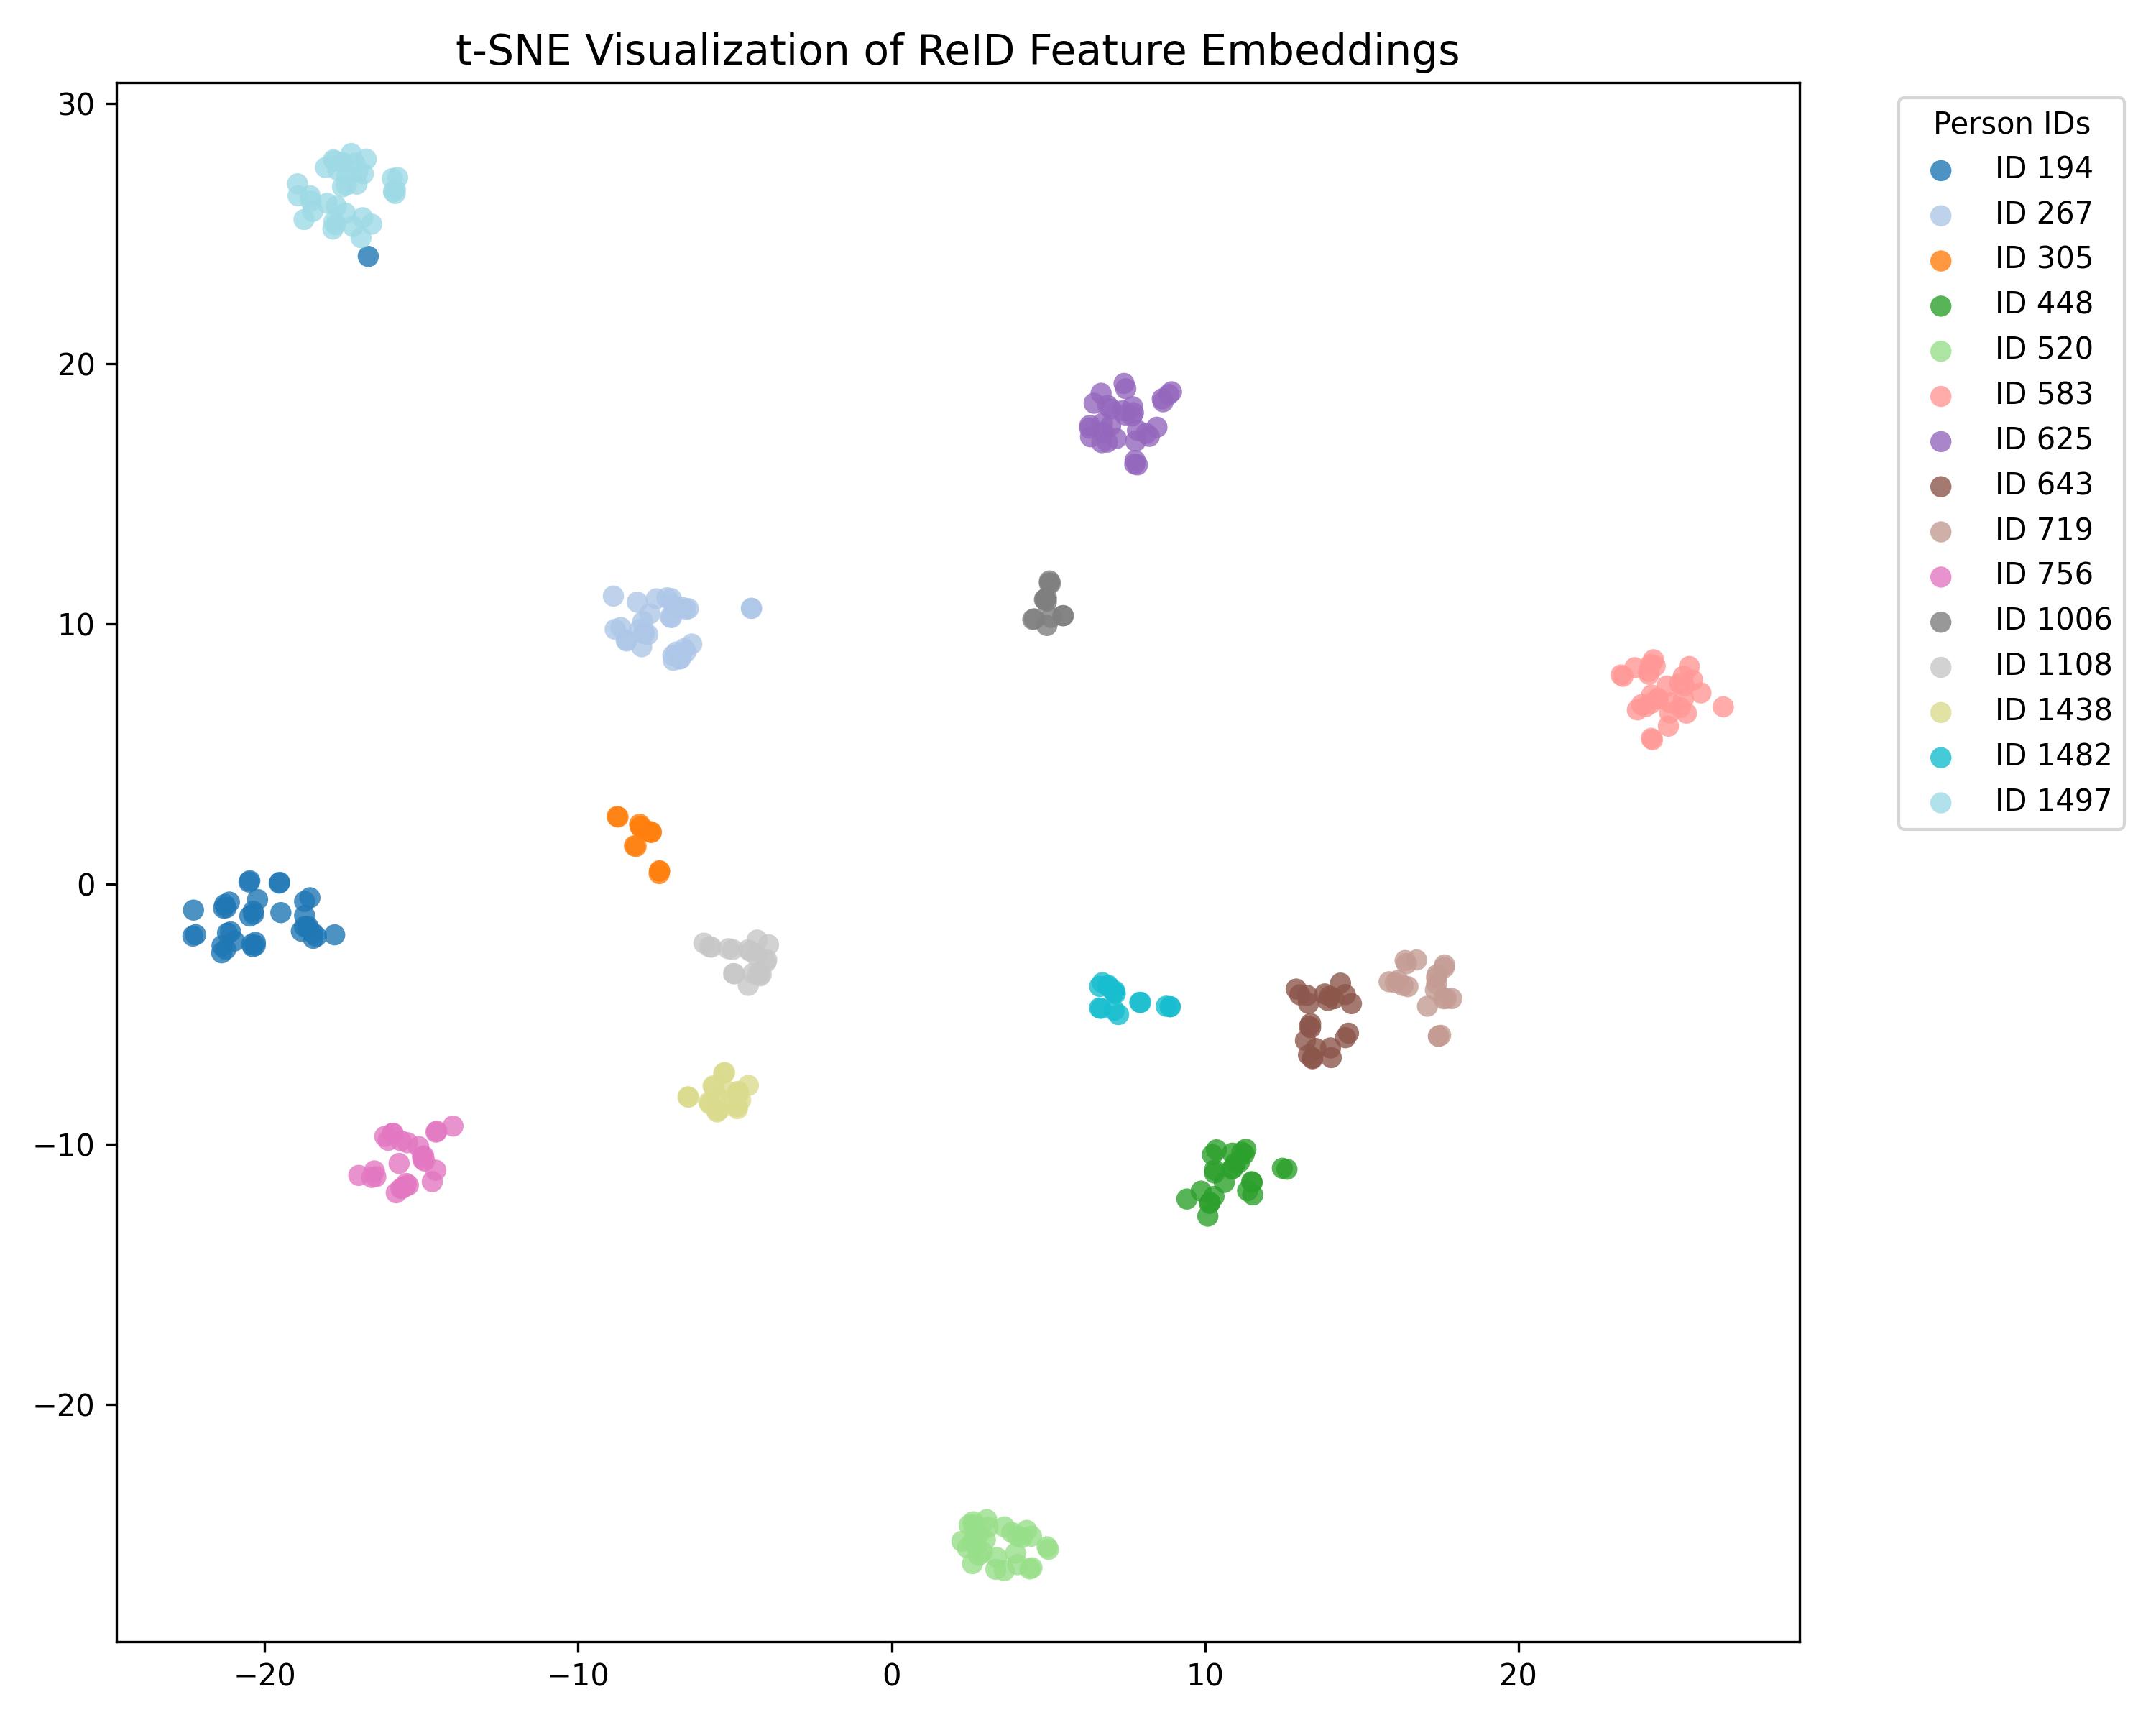
\includegraphics[width=0.45\linewidth,height=0.40\textheight,keepaspectratio]{tsne/tsne_plot.png}
        \hspace{0.04\linewidth}
        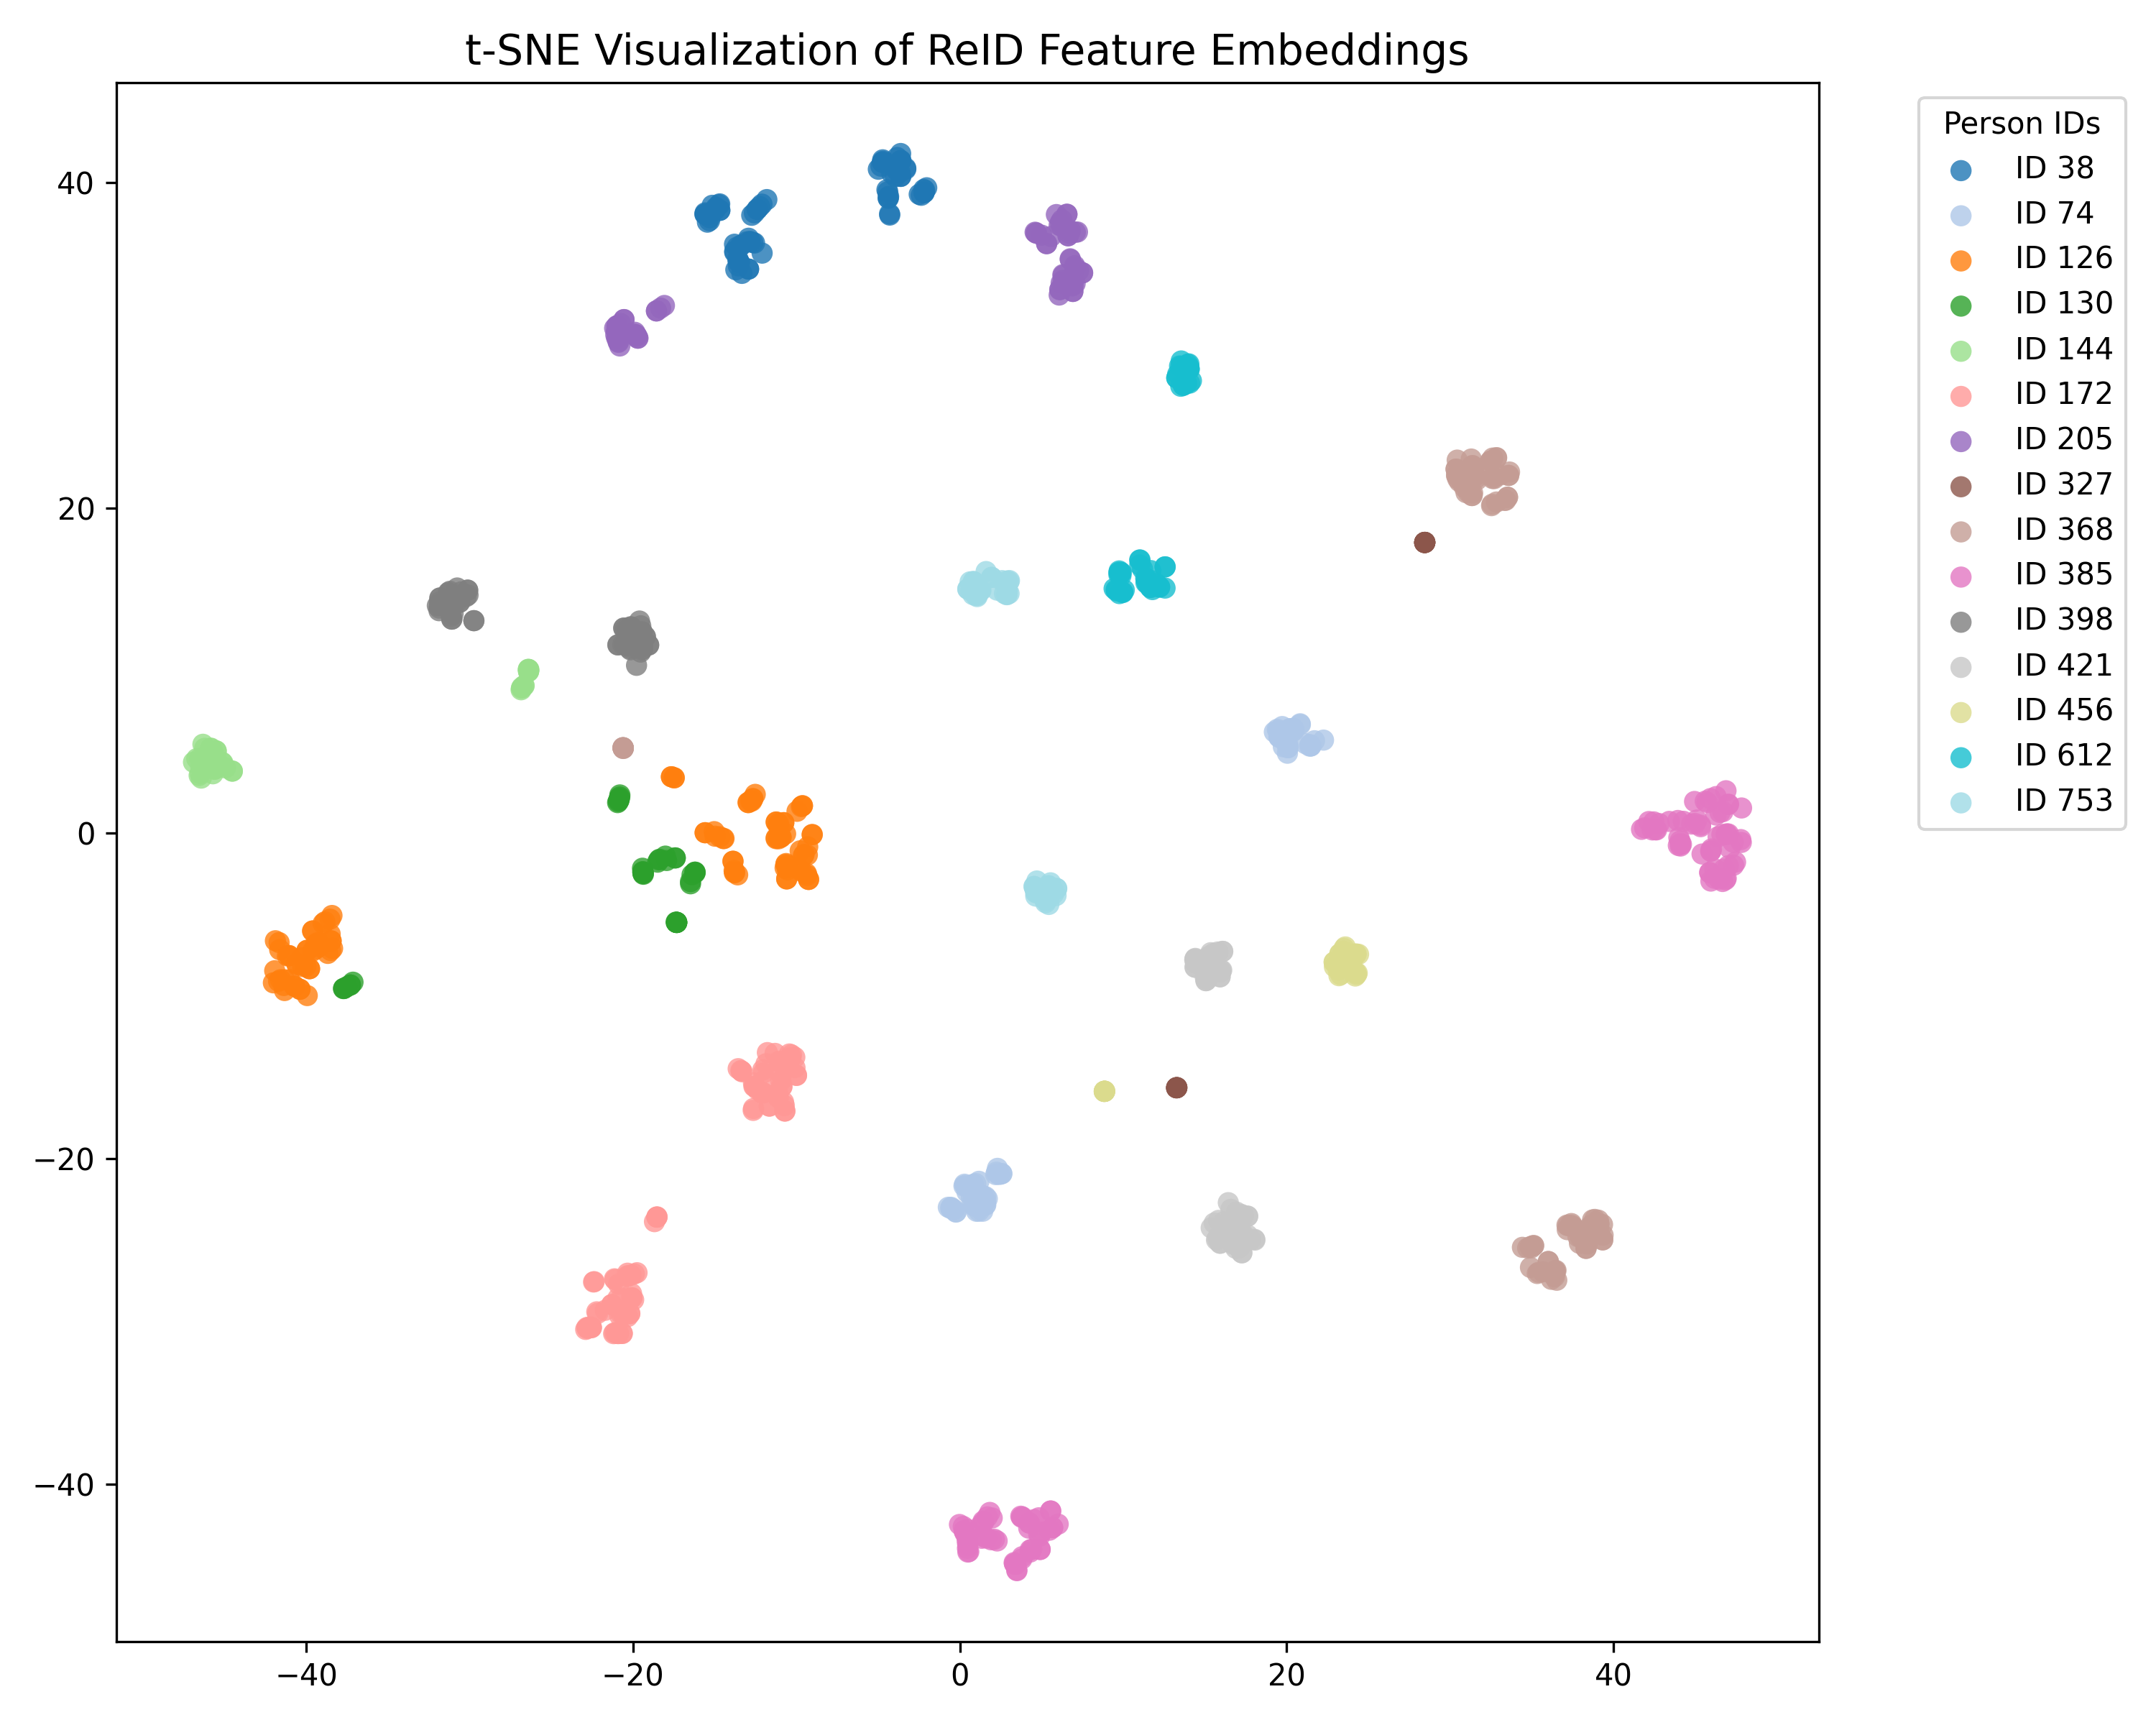
\includegraphics[width=0.45\linewidth,height=0.40\textheight,keepaspectratio]{veri/tsne/tsne_plot.png}
    \end{center}
    \vspace{-0.3em}
    \footnotesize
    \textbf{Hyperspherical Clustering}: Normalized chordal metric learning forms compact intra-identity clusters and wide inter-camera separation margins across diverse viewpoints.
\end{column}
\end{columns}
\end{frame}

% -------------------------------------------------------------
% Slide 18: Summary of Contributions, Conclusion & Discussion
% -------------------------------------------------------------
\begin{frame}{Summary of Contributions, Conclusion \& Discussion}
\begin{columns}[t,onlytextwidth]
\begin{column}{0.32\textwidth}
    \footnotesize
    \textbf{Theoretical Diagnosis}
    \begin{itemize}
        \setlength{\itemsep}{0.12em}
        \scriptsize
        \item \textbf{Theorems 1--5}: Formalized gradient sign inversion, supervision polarity inversion, triplet saturation, grid collapse, and score floors.
        \item \textbf{Proposition 1}: Proved non-singularity ($\det(\mathbf{A}) \ge 0.196$) and 0.0\% padding.
        \item Established mathematical grounding for parameter diffusion.
    \end{itemize}
\end{column}
\begin{column}{0.32\textwidth}
    \footnotesize
    \textbf{Optimization Suite}
    \begin{itemize}
        \setlength{\itemsep}{0.12em}
        \scriptsize
        \item \textbf{Architectural Refinement}: Non-singular STN + lightweight MLP (96.5\% VRAM reduction).
        \item \textbf{Sampling Refinement}: 5-step analytic DDIM reverse trajectory.
        \item \textbf{Regularizations}: Detached softmax, Gaussian MMD, chordal metric.
    \end{itemize}
\end{column}
\begin{column}{0.32\textwidth}
    \footnotesize
    \textbf{Empirical Impact}
    \begin{itemize}
        \setlength{\itemsep}{0.12em}
        \scriptsize
        \item \textbf{Market-1501}: 85.6\% base mAP (89.8\% with re-ranking).
        \item \textbf{VeRi-776}: 52.4\% base mAP (54.1\% with re-ranking, +10.1\% gain).
        \item \textbf{Near-Optimality}: Within 2.6\% of supervised ceiling (88.2\%) with narrow variance ($\sigma=0.28\%$).
    \end{itemize}
\end{column}
\end{columns}

\vspace{0.4em}
\footnotesize
\textbf{Key Takeaway}: Parameter-space diffusion acts as a potent geometric prior once mathematical bottlenecks are resolved. \hfill \textbf{Thank You! (Q\&A)}
\end{frame}

\end{document}
